\section{总体、样本与统计量}
\subsection{总体与样本}
\textbf{总体}：研究对象的全体。通常指研究对象的某项数量指标。组成总体的元素称为个体。从本质上讲，总体就是所研究的随机变量或随机变量的分布。

\textbf{样本}：来自总体的部分个体 $\mathbf{X}_1, \dots, \mathbf{X}_n$。如果满足：
\begin{enumerate}
	\item 同分布性：$\mathbf{X}_i\ (i=1,\dots,n)$ 与总体同分布。
	\item 独立性：$\mathbf{X}_1, \dots, \mathbf{X}_n$ 相互独立。
\end{enumerate}
则称为容量为 $n$ 的简单随机样本，简称样本。而称 $\mathbf{X}_1, \dots, \mathbf{X}_n$ 的一次实现为样本观察值，记为 $\mathbf{x}_1, \dots, \mathbf{x}_n$。

来自总体 $X$ 的随机样本 $\mathbf{X}_1, \cdots, \mathbf{X}_n$ 可记为
\begin{equation}
	X_1, \cdots, X_n \overset{iid}{\sim} X \quad \text{或} \quad f(x),\, F(x),\, \dots
	\label{eq:基本概念:样本记号}
\end{equation}

显然，样本联合分布函数或密度函数为
\begin{equation}
	F^*(x_1, x_2, \cdots, x_n) = \prod_{i=1}^{n} F(x_i)
	\label{eq:基本概念:联合分布函数}
\end{equation}
或
\begin{equation}
	f^*(x_1, x_2, \cdots, x_n) = \prod_{i=1}^{n} f(x_i)
	\label{eq:基本概念:联合密度}
\end{equation}

\subsection{统计量}
称样本 $X_1, \cdots, X_n$ 的函数 $g(X_1, \cdots, X_n)$ 是总体 $X$ 的一个 \textcolor{red}{统计量}，如果 $g(X_1, \cdots, X_n)$ \textcolor{red}{不含未知参数}。

\textbf{几个常用的统计量：}
\begin{enumerate}
	\item 样本均值（Sample Mean）：
	\begin{equation}
		\bar{X} = \frac{1}{n} \sum_{i=1}^{n} X_i
		\label{eq:基本概念:样本均值}
	\end{equation}
	\item 样本方差（Sample Variance）：
	\begin{equation}
		S^2 = \frac{1}{n-1} \sum_{i=1}^{n} (X_i - \bar{X})^2
		\label{eq:基本概念:样本方差}
	\end{equation}
	注意：这里的系数是 $\frac{1}{n-1}$ 而不是 $\frac{1}{n}$，这是为了保证它是无偏估计量。
	\item 样本均方差（标准差，Sample Standard Deviation）：
	\begin{equation}
		S = \sqrt{S^2}
		\label{eq:基本概念:样本标准差}
	\end{equation}
	\item 样本 $k$ 阶矩：
	\begin{itemize}
		\item 样本原点矩（Sample Moment about Origin）：
		\begin{equation}
			\frac{1}{n} \sum_{i=1}^{n} X_i^k
			\label{eq:基本概念:原点矩}
		\end{equation}
		注：当 $k=1$ 时，这就是样本均值。
		\item 样本中心矩（Sample Central Moment）：
		\begin{equation}
			\frac{1}{n} \sum_{i=1}^{n} (X_i - \bar{X})^k
			\label{eq:基本概念:中心矩}
		\end{equation}
		注：当 $k=2$ 时，这对应于样本方差的某种形式，但通常样本方差分母为 $n-1$。
	\end{itemize}
	\item 经验分布函数（Empirical Distribution Function）：用 $S(x)$ 表示样本 $X_1, \cdots, X_n$ 中\textbf{不大于 $x$} 的随机变量个数，定义经验分布函数 $F_n(x)$ 为：
	\begin{equation}
		F_n(x) = \frac{1}{n} S(x)
		\label{eq:基本概念:经验分布函数}
	\end{equation}
\end{enumerate}

\section{常用统计量的分布（抽样分布）}
\subsection{$\chi^2$ 分布}
\textbf{1. 构造}：设 $X_1, \cdots, X_n$ 独立同分布于标准正态分布，即 $X_1, \cdots, X_n \overset{iid}{\sim} N(0,1)$，则定义统计量
\begin{equation}
	\chi^2 = \sum_{i=1}^{n} X_i^2 \sim \chi^2(n)
	\label{eq:抽样分布:卡方构造}
\end{equation}
称为\textbf{自由度为 $n$ 的 $\chi^2$ 分布}。

\begin{myhypothesis}{笔记要点}
	$\chi^2$ 分布本质上就是 $n$ 个独立的标准正态随机变量的平方和。
\end{myhypothesis}

\textbf{2. $\chi^2$ 分布的概率密度函数}：
\begin{equation}
	f(y) = \begin{cases} \dfrac{1}{2^{n/2}\Gamma(n/2)}\, y^{\frac{n}{2}-1}\, e^{-\frac{y}{2}}, & y > 0 \\[1ex] 0, & y \le 0 \end{cases}
	\label{eq:抽样分布:卡方密度}
\end{equation}
其中 $\Gamma(\cdot)$ 是伽马函数。

\begin{center}
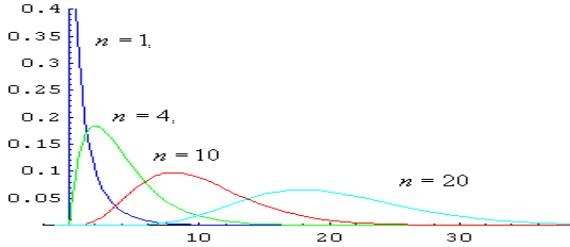
\includegraphics[width=0.55\linewidth]{Figures/chi2_density.png}
\end{center}

\textbf{特点}：分布是非对称的（右偏），取值恒为正。随着自由度 $n$ 的增大，曲线峰值向右移动，且图形逐渐趋向于对称（正态分布）。

\textbf{3. $\chi^2$ 分布的分位点}：设 $X \sim \chi^2(n)$，若对于 $\alpha: 0 < \alpha < 1$，存在 $\chi^2_{\alpha}(n) > 0$ 满足：
\begin{equation}
	P\{X \ge \chi^2_{\alpha}(n)\} = \alpha
	\label{eq:抽样分布:卡方分位点}
\end{equation}
则称 $\chi^2_{\alpha}(n)$ 为 $\chi^2(n)$ 分布的\textbf{上 $\alpha$ 分位点}（Upper $\alpha$ quantile）。

\begin{center}
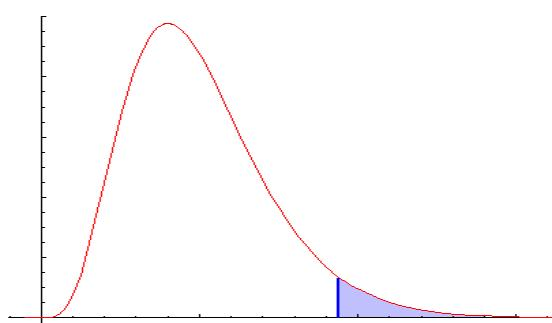
\includegraphics[width=0.55\linewidth]{Figures/chi2_quantile.png}
\end{center}

\textbf{图示说明}：
\begin{itemize}
	\item 图中阴影部分的面积为 $\alpha$（右尾概率）。
	\item $\chi^2_{\alpha}(n)$ 是横轴上的临界值。
\end{itemize}

举例：
\begin{itemize}
	\item $\chi^2_{0.05}(10) = 18.307$（表示自由度为10时，大于18.307的概率是0.05）
	\item $\chi^2_{0.95}(10) = 3.940$（表示自由度为10时，大于3.940的概率是0.95）
\end{itemize}

\textbf{4. $\chi^2$ 分布的性质}：
\begin{enumerate}[label=(\alph*)]
	\item 分布可加性（Additivity）：若 $X \sim \chi^2(n_1)$，$Y \sim \chi^2(n_2)$，且 $X, Y$ 相互独立，则它们的和服从自由度相加的 $\chi^2$ 分布：
	\begin{equation}
		X + Y \sim \chi^2(n_1 + n_2)
		\label{eq:抽样分布:卡方可加性}
	\end{equation}
	\item 期望与方差（Expectation and Variance）：若 $X \sim \chi^2(n)$，则
	\begin{itemize}
		\item \textbf{期望}：$E(X) = n$
		\item 方差：$D(X) = 2n$（记忆技巧：期望等于自由度，方差等于两倍自由度）
	\end{itemize}
\end{enumerate}

\subsection{$t$ 分布}
\textbf{1. 构造（Construction）}：这是 $t$ 分布最经典的定义方式，一定要背下来：
\begin{itemize}
	\item 设 $\xi \sim N(0, 1)$（$\xi$ 是标准正态分布）
	\item 设 $\eta \sim \chi^2(n)$（$\eta$ 是自由度为 $n$ 的卡方分布）
	\item 且 $\xi$ 与 $\eta$ 相互独立
\end{itemize}
则构造出的统计量 $T$ 为：
\begin{equation}
	T = \frac{\xi}{\sqrt{\eta / n}} \sim t(n)
	\label{eq:抽样分布:t构造}
\end{equation}
称 $t(n)$ 为\textbf{自由度为 $n$ 的 $t$ 分布}。

\textbf{$t$ 分布的直观理解}：
\begin{itemize}
	\item 分子是一个\textbf{标准正态变量}。
	\item 分母是一个\textbf{调整后的卡方变量的平方根}（起到了"归一化"或"缩放"的作用）。
	\item 当样本量 $n \to \infty$ 时，$t$ 分布会收敛于标准正态分布 $N(0,1)$。但在小样本下，$t$ 分布的尾部比正态分布更"厚"（更平坦），这使得它在小样本估计中更为保守和准确。
\end{itemize}

\textbf{2. $t(n)$ 的概率密度}：
\begin{equation}
	f(t) = \frac{\Gamma\left(\frac{n+1}{2}\right)}{\sqrt{n\pi}\,\Gamma\left(\frac{n}{2}\right)} \left(1+\frac{t^2}{n}\right)^{-\frac{n+1}{2}}, \quad -\infty < t < \infty
	\label{eq:抽样分布:t密度}
\end{equation}

\textbf{公式组成}：
\begin{itemize}
	\item $\Gamma(\cdot)$：这是伽马函数（Gamma Function，欧拉第二积分），它是阶乘在实数域上的推广。
	\item $\left(1+\frac{t^2}{n}\right)^{-\frac{n+1}{2}}$：这是函数的主体部分，是一个幂函数形式，它决定了 $t$ 分布呈钟形曲线，且比正态分布下降得更慢（即"厚尾"）。
\end{itemize}

\textbf{3. 基本性质}：
\begin{center}
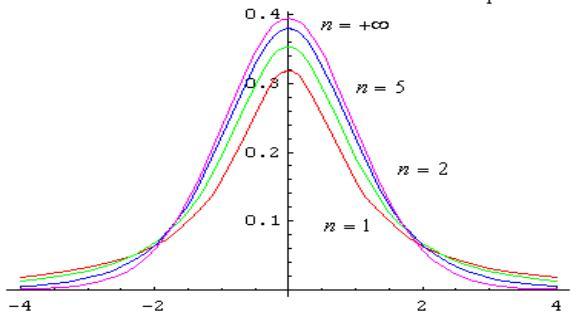
\includegraphics[width=0.55\linewidth]{Figures/t_properties.png}
\end{center}
\begin{enumerate}
	\item \textbf{对称性}：$f(t)$ 关于 $t=0$（纵轴）对称。
	\item 极限性质：当自由度 $n \to \infty$ 时，$f(t)$ 的极限是标准正态分布 $N(0, 1)$ 的密度函数，即
	\begin{equation}
		\lim_{n \to \infty} f(t) = \varphi(t) = \frac{1}{\sqrt{2\pi}} e^{-\frac{t^2}{2}}, \quad -\infty < t < \infty
		\label{eq:抽样分布:t极限}
	\end{equation}
\end{enumerate}

\textbf{4. 分位点}：设 $T \sim t(n)$，若对于 $\alpha: 0 < \alpha < 1$，存在 $t_\alpha(n)$，满足：
\begin{equation}
	P\{T \ge t_\alpha(n)\} = \alpha
	\label{eq:抽样分布:t分位点}
\end{equation}
则称 $t_\alpha(n)$ 为 $t(n)$ 分布的上侧 $\alpha$ 分位点。

\textbf{重点性质：分位点的对称性}——由于 $t$ 分布关于 $t=0$ 对称，因此
\begin{equation}
	t_{1-\alpha}(n) = -t_{\alpha}(n)
	\label{eq:抽样分布:t分位点对称性}
\end{equation}

\textbf{示例}：
\begin{itemize}
	\item $t_{0.01}(20) = 2.5280$
	\item $t_{0.99}(20) = t_{1-0.01}(20) = -t_{0.01}(20) = -2.5280$
\end{itemize}

\subsection{$F$ 分布}
\textbf{1. 构造}：$F$ 分布是通过两个独立的卡方（$\chi^2$）随机变量的比值构造而成的。设 $\eta_1$ 和 $\eta_2$ 是两个独立的卡方随机变量，其自由度分别为 $n_1$ 和 $n_2$：
\begin{itemize}
	\item $\eta_1 \sim \chi^2(n_1)$
	\item $\eta_2 \sim \chi^2(n_2)$
\end{itemize}
则随机变量 $F$ 的构造如下：
\begin{equation}
	F = \frac{\eta_1/n_1}{\eta_2/n_2} \sim F(n_1, n_2)
	\label{eq:抽样分布:F构造}
\end{equation}
\textbf{自由度}：$n_1$ 称为\textbf{第一自由度}（分子自由度），$n_2$ 称为\textbf{第二自由度}（分母自由度）。

\textbf{2. 概率密度函数}：对于 $F(n_1, n_2)$ 分布，其概率密度函数 $h(y)$ 如下（其中 $\Gamma$ 是伽马函数）：
\begin{equation}
	h(y) = \begin{cases} \dfrac{\Gamma\left(\frac{n_1+n_2}{2}\right) \left(n_1/n_2\right)^{n_1/2}}{\Gamma\left(\frac{n_1}{2}\right) \Gamma\left(\frac{n_2}{2}\right)} \cdot \dfrac{y^{\frac{n_1}{2}-1}}{\left(1+\frac{n_1}{n_2}y\right)^{(n_1+n_2)/2}}, & y > 0 \\[1ex] 0, & y \le 0 \end{cases}
	\label{eq:抽样分布:F密度}
\end{equation}

\textbf{3. $F$ 分布的分位点}：对于一个概率 $\alpha$（$0 < \alpha < 1$），如果存在一个正数 $F_{\alpha}(n_1, n_2)$，使得随机变量 $F$ 大于或等于该值的概率恰好是 $\alpha$，则称 $F_{\alpha}(n_1, n_2)$ 为 $F(n_1, n_2)$ 分布的上侧 $\alpha$ 分位点。
\begin{equation}
	P\{F \ge F_{\alpha}(n_1, n_2)\} = \alpha
	\label{eq:抽样分布:F分位点}
\end{equation}

\textbf{4. 分位点的性质}：下侧分位点与上侧分位点之间的关系：
\begin{equation}
	F_{1-\alpha}(n_1, n_2) = \frac{1}{F_{\alpha}(n_2, n_1)}
	\label{eq:抽样分布:F分位点性质}
\end{equation}

\section{正态总体下的三大抽样定理}
\begin{myTheorem}{定理一：标准化样本均值的分布（$U$ 统计量）}
	\textbf{结论}：当总体方差 $\sigma^2$ \textbf{已知}时，标准化后的样本均值服从标准正态分布 $N(0, 1)$。
	\begin{equation}
		U = \frac{\bar{X} - \mu}{\sigma/\sqrt{n}} \sim N(0, 1)
		\label{eq:抽样定理:U}
	\end{equation}
	\textbf{用途}：用于总体均值 $\mu$ 的大样本检验，或 $\sigma^2$ 已知时的单样本检验。
\end{myTheorem}

\begin{myTheorem}{定理二：样本方差的分布（$\chi^2$ 统计量）}
	\textbf{结论}：将样本方差 $S^2$ 乘以适当的系数后，服从自由度为 $n-1$ 的 $\chi^2$ 分布（卡方分布）。
	\begin{equation}
		\chi^2 = \frac{(n-1)S^2}{\sigma^2} \sim \chi^2(n-1)
		\label{eq:抽样定理:卡方}
	\end{equation}
	\textbf{用途}：用于总体方差 $\sigma^2$ 的估计和检验。
\end{myTheorem}

\begin{myTheorem}{定理三：$t$ 统计量的分布（小样本下的均值检验）}
	\textbf{结论}：当总体方差 $\sigma^2$ \textbf{未知}时，使用样本标准差 $S$ 替代 $\sigma$ 对 $\bar{X}$ 进行标准化，得到的统计量服从自由度为 $n-1$ 的 $t$ 分布。
	\begin{equation}
		T = \frac{\bar{X} - \mu}{S/\sqrt{n}} \sim t(n-1)
		\label{eq:抽样定理:T}
	\end{equation}
	\textbf{用途}：用于总体均值 $\mu$ 的小样本检验，或 $\sigma^2$ 未知时的单样本检验。
\end{myTheorem}

\subsection{附加重要结论}
\textbf{独立性结论}：在正态总体下，样本均值 $\bar{X}$ 与样本方差 $S^2$ 相互独立。（这是构建 $T$ 统计量的关键，因为 $T$ 统计量的构造要求分子（$U$）和分母的平方根（$\sqrt{\chi^2/n}$）相互独立。）

\textbf{延伸：两个正态总体的方差比（$F$ 统计量）}：$F$ 分布是这三大定理的自然延伸，它用于比较两个独立正态总体的方差。设有两个独立样本，来自 $N(\mu_1, \sigma_1^2)$ 和 $N(\mu_2, \sigma_2^2)$：
\begin{equation}
	F = \frac{S_1^2 / \sigma_1^2}{S_2^2 / \sigma_2^2} \sim F(n_1-1, n_2-1)
	\label{eq:抽样定理:F}
\end{equation}
\textbf{用途}：用于检验两个总体的方差是否相等（即检验 $H_0: \sigma_1^2 = \sigma_2^2$）。
